%%% MORITZ 5' %%%

\section{Bestimmung der Relaxationszeit nach Franzen}
\subsection{Grundlagen}

\begin{frame}
\frametitle{Grundlagen: Bestimmung der Relaxationszeit nach Franzen}

\setbeamerfont{myfont}{size*=80}
\usebeamerfont{myfont}
\begin{figure}
    \centering
    \def\svgwidth{\textwidth}
    \input{../img/FranzenTheo0.pdf_tex}
    \caption{Theoretischer Verlauf der Transmission bei der Messmethode nach Franzen.}
\end{figure}

  
\end{frame}


\begin{frame}[noframenumbering]
\frametitle{Grundlagen: Bestimmung der Relaxationszeit nach Franzen}

\setbeamerfont{myfont}{size*=80}
\usebeamerfont{myfont}
\addtocounter{figure}{-1}
\begin{figure}
    \centering
    \def\svgwidth{\textwidth}
    \input{../img/FranzenTheo.pdf_tex}
    \caption{Theoretischer Verlauf der Transmission bei der Messmethode nach Franzen.}
\end{figure}

  
\end{frame}

\subsection{Aufbau}
\begin{frame}
\frametitle{Aufbau: Bestimmung der Relaxationszeit nach Franzen}

\setbeamerfont{myfont}{size*=80}
\usebeamerfont{myfont}
\begin{figure}
    \centering
    \def\svgwidth{\textwidth}
    \input{../img/aufbaufranzen.pdf_tex}
    \caption{Aufbau zur Bestimmung der Relaxationszeit nach Franzen.}
\end{figure}
\usebeamerfont{standard}

\begin{itemize}
  \item \textbf{Chopper:} Periodische Unterbrechung des Laserlichts
  \item \textbf{Spule 1:} Kompensation von horizontalem Erdmagnetfeld
  \item \textbf{Spule 4:} Kompensation von vertikalem Erdmagnetfeld
\end{itemize}

\end{frame}

\subsection{Auswertung}
\begin{frame}
\frametitle{Auswertung: Bestimmung der Relaxationszeit nach Franzen}

\begin{figure}
    \centering
    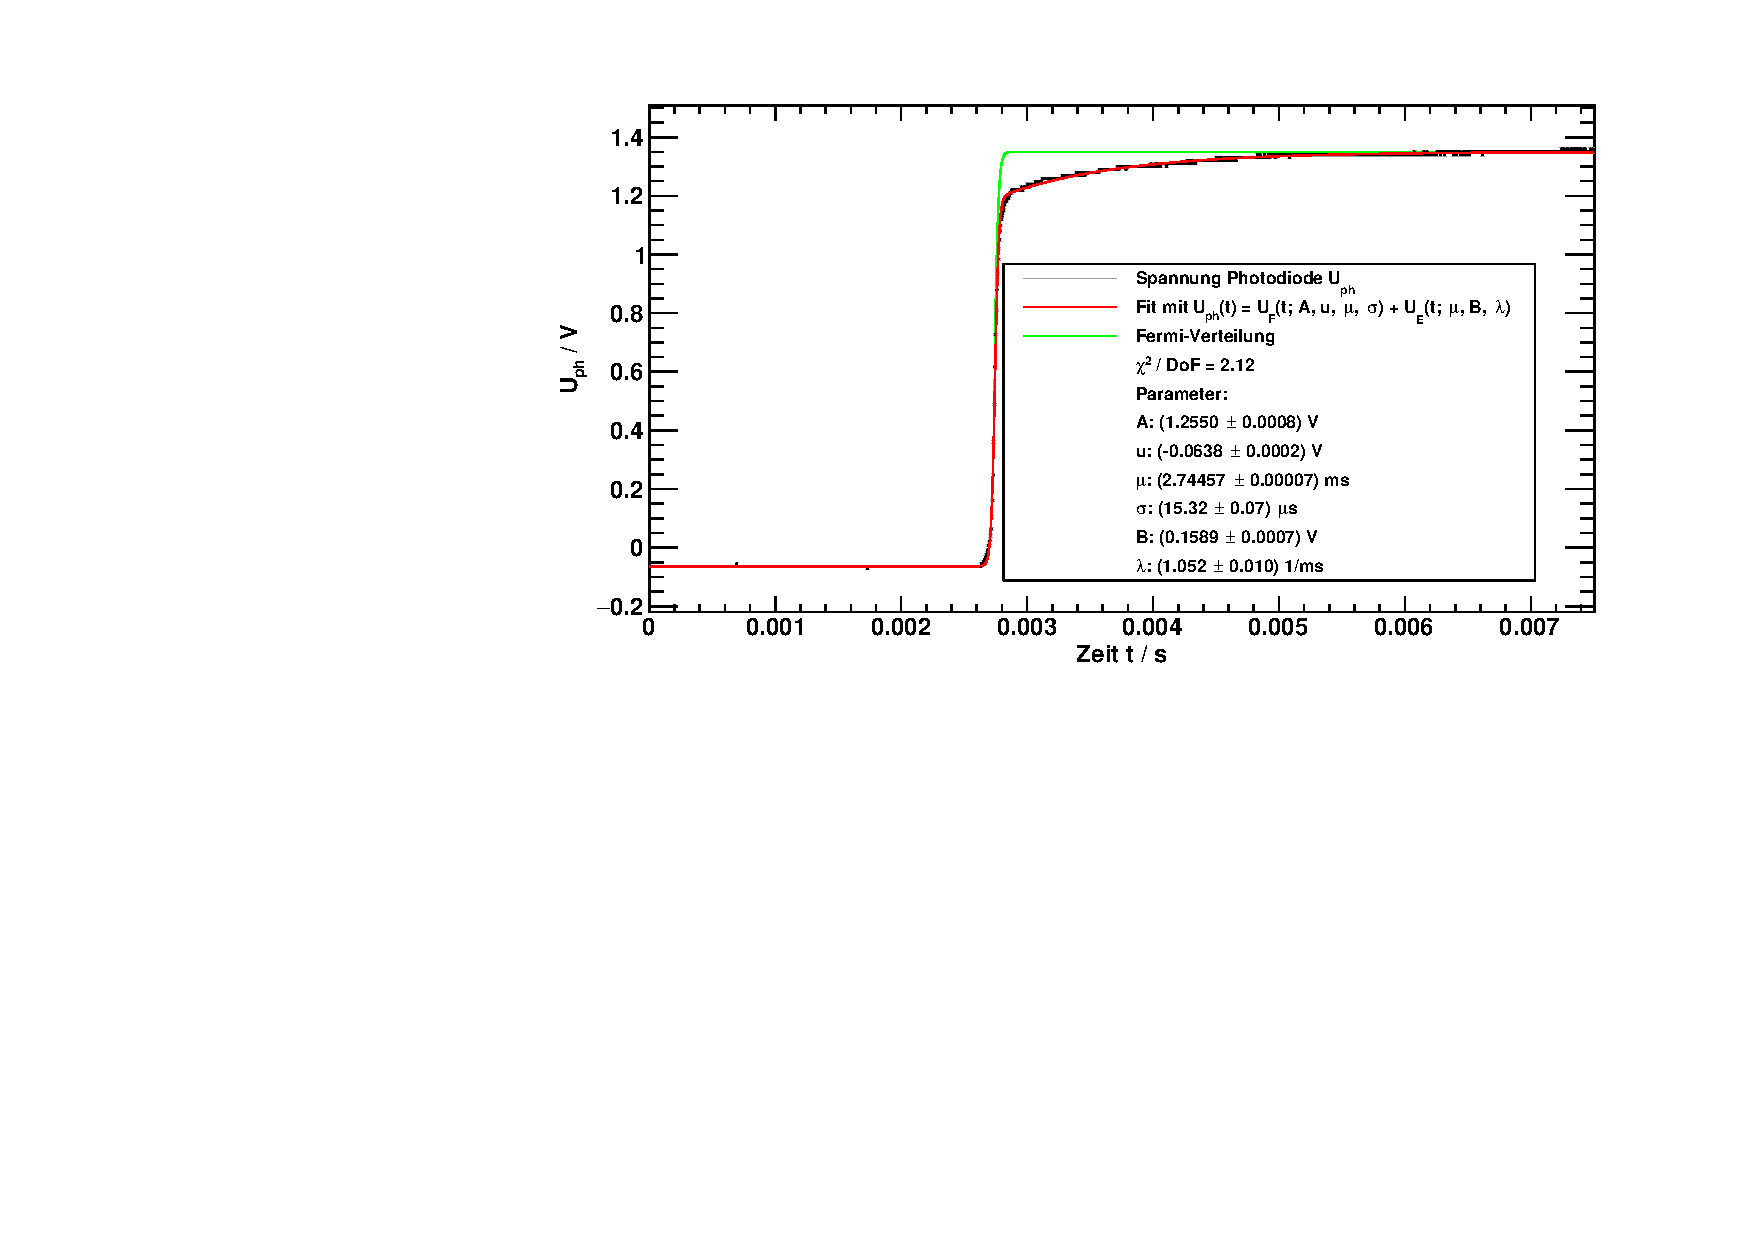
\includegraphics[width=\textwidth]{../img/04.pdf}
    \caption{Transmission der Messzelle nach Öffnung des Strahlengangs.}  
\end{figure} 
  
\end{frame}


\begin{frame}
\frametitle{Auswertung: Bestimmung der Relaxationszeit nach Franzen}

\begin{figure}
    \centering
    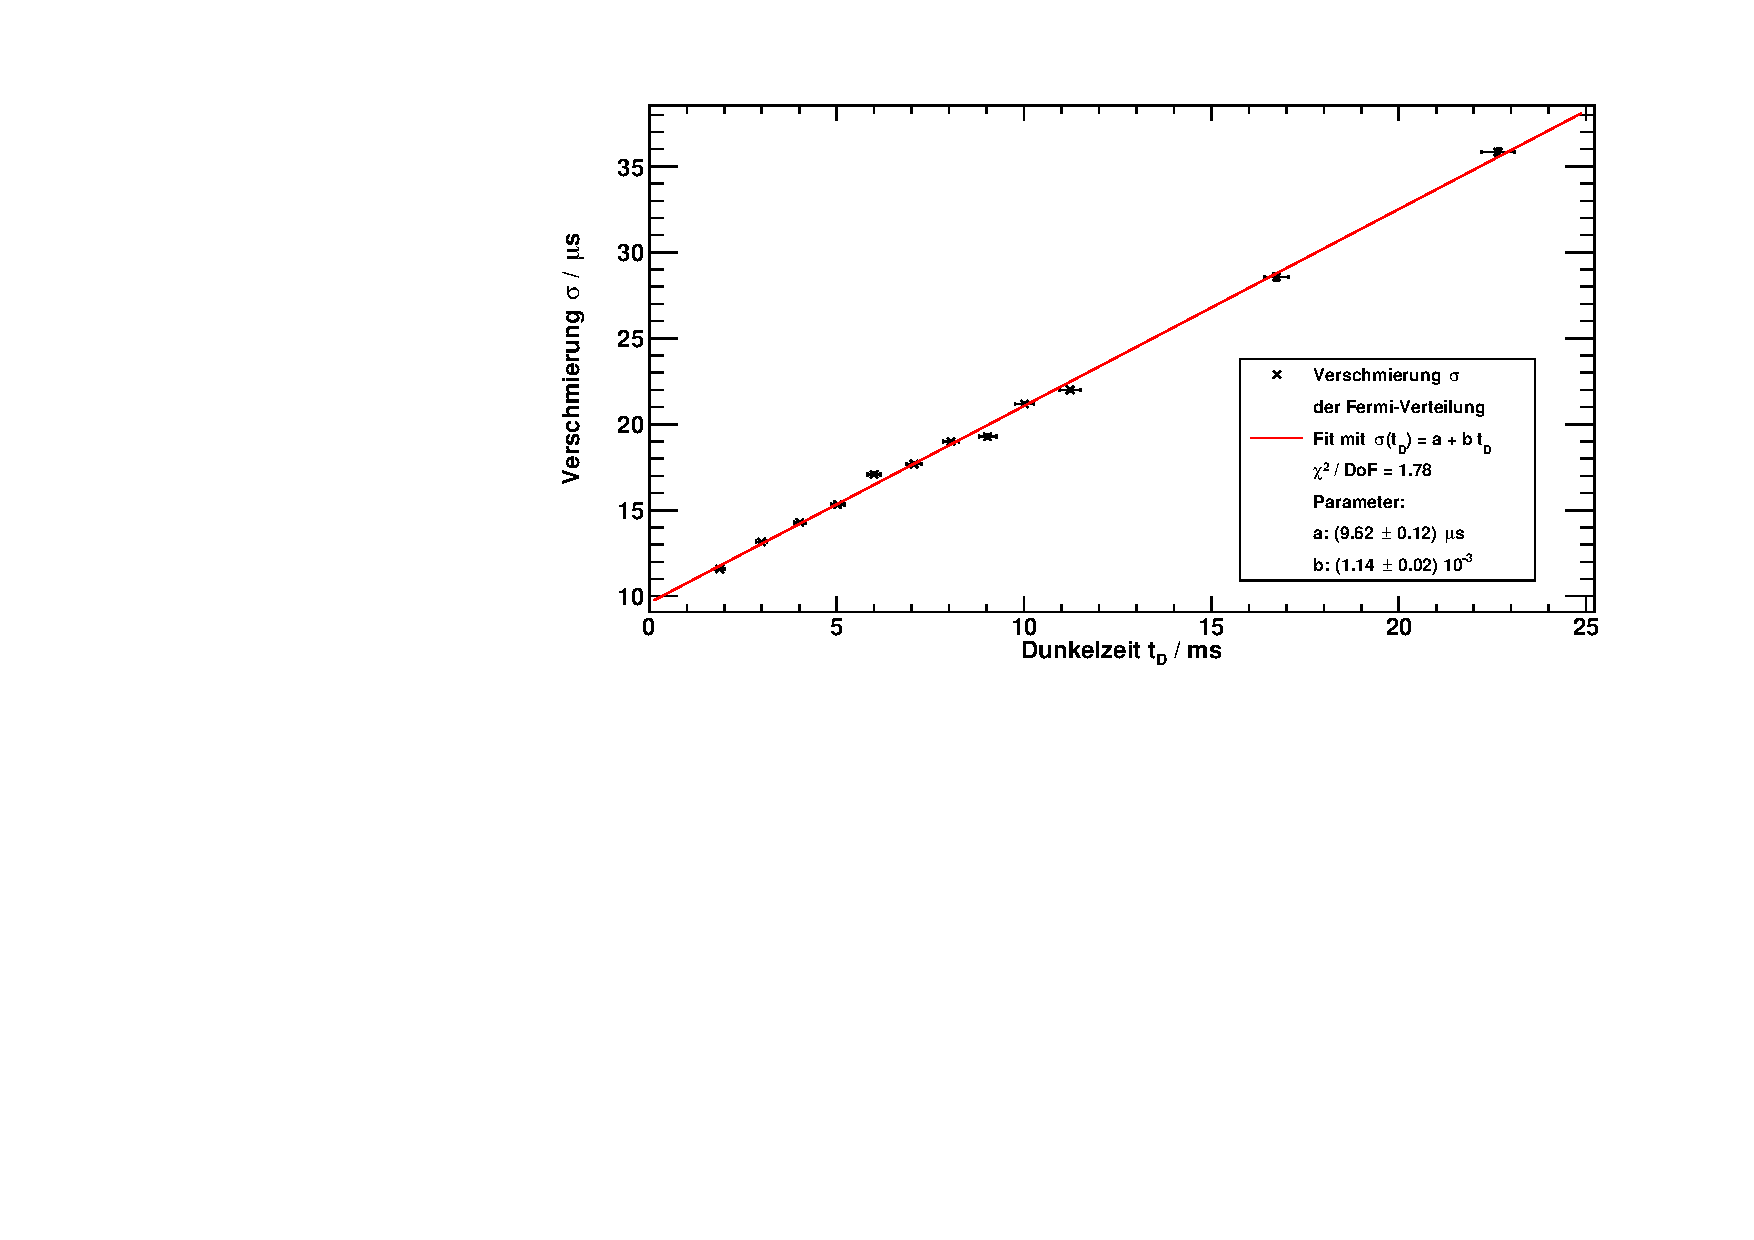
\includegraphics[width=\textwidth]{../img/sigmaFit.pdf}
    \caption{Abrundung $\sigma$ der gefitteten Fermi-Funktionen.}  
\end{figure} 
  
\end{frame}


\begin{frame}
\frametitle{Auswertung: Bestimmung der Relaxationszeit nach Franzen}

\begin{figure}
    \centering
    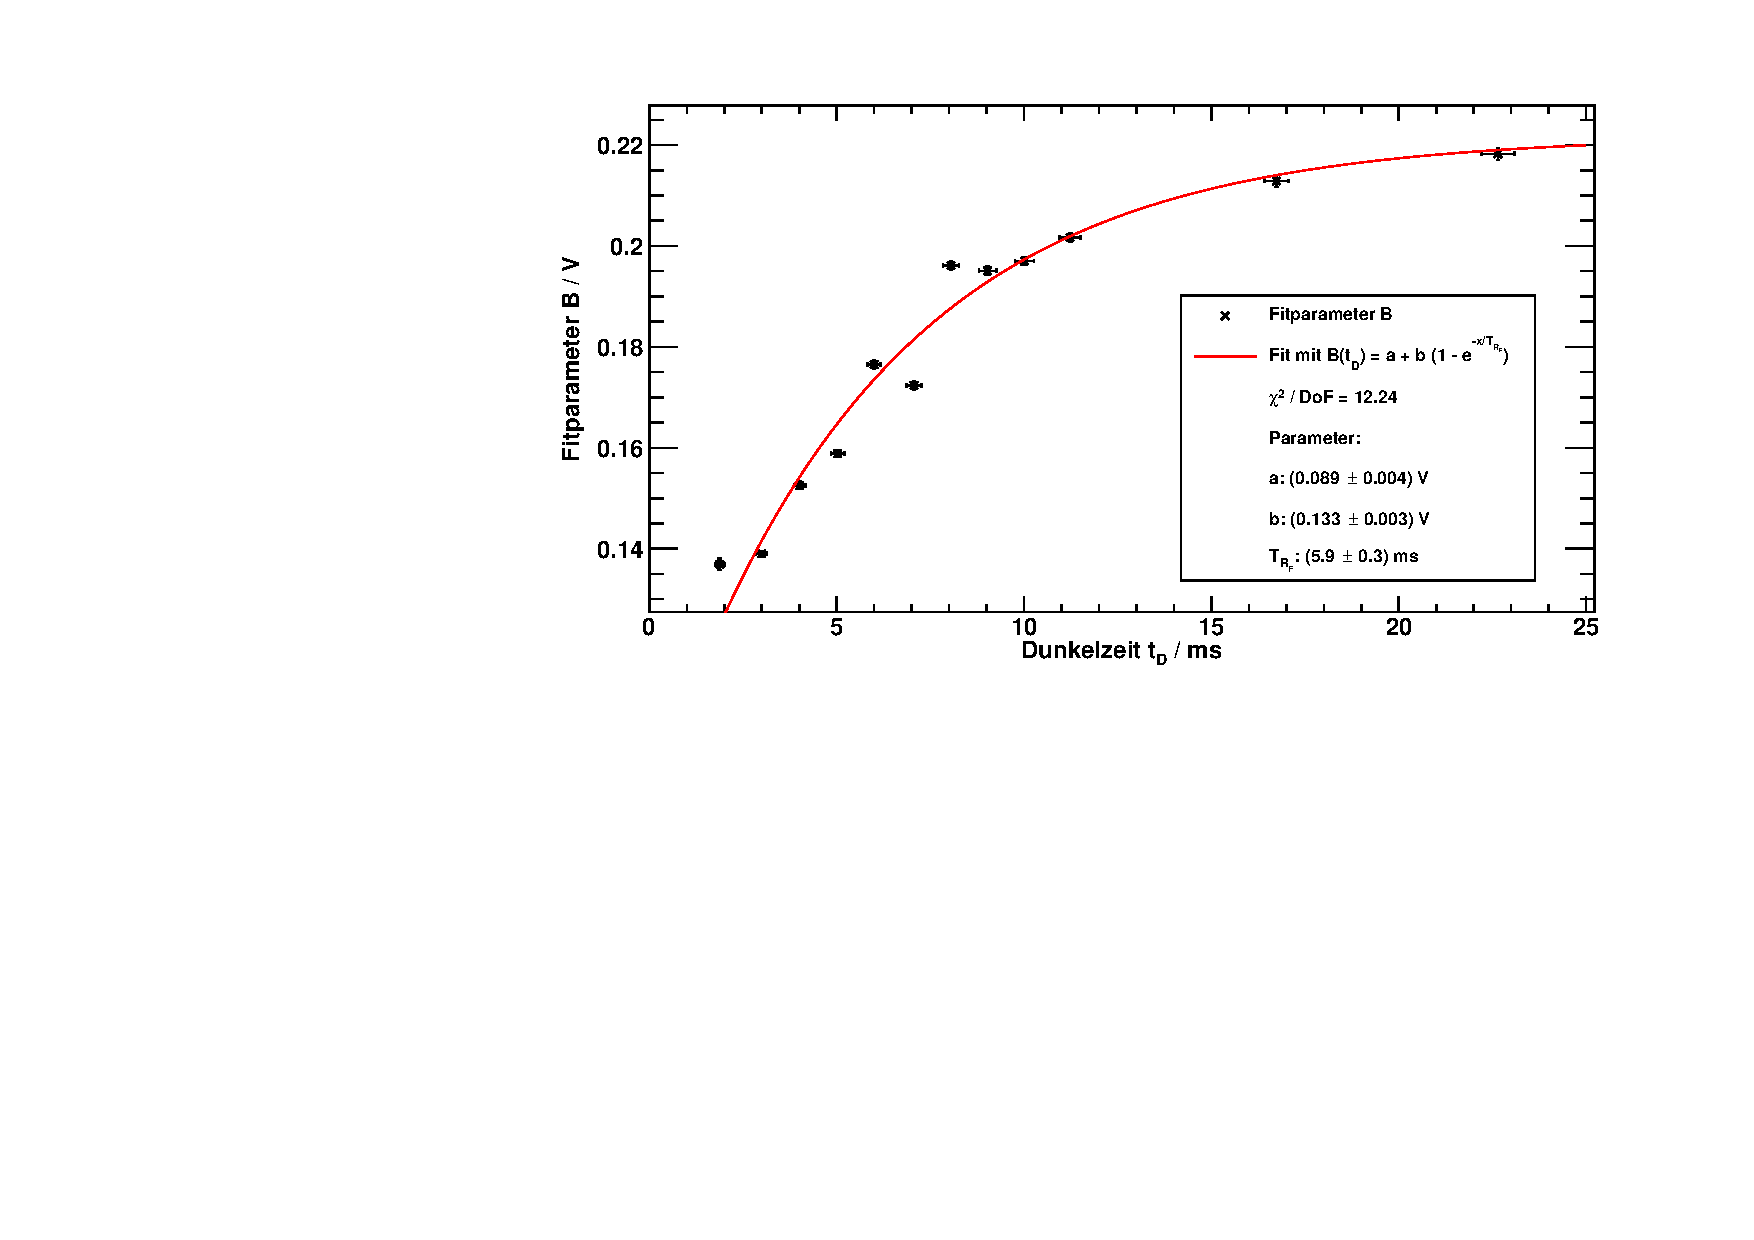
\includegraphics[width=\textwidth]{../img/BFit.pdf}
    \caption{Startwerte der gefitteten Exponentialfunktionen.}  
\end{figure} 
  
\end{frame}


\begin{frame}
\frametitle{Ergebnis: Bestimmung der Relaxationszeit nach Franzen}
\begin{itemize}
    \item Relaxationszeit
    \begin{equation*}
        T_{\text{R}_\text{F}} = 5.9 \pm 0.3\,\text{ms}
    \end{equation*}
    \item Literaturwert
    \begin{equation*}
        T_{\text{R}}^\text{Lit.} = 6.5\,\text{ms}
    \end{equation*}
\end{itemize}
  
\end{frame}